\subsubsection{UC4 - Registrazione}
\begin{figure}[h]
	\centering
	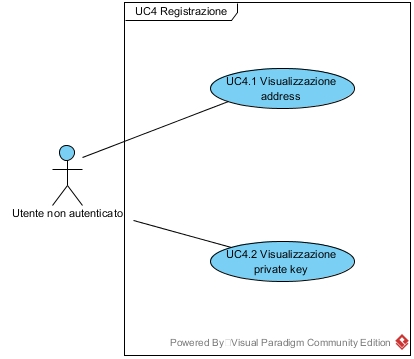
\includegraphics[width=0.7\linewidth]{res/img/UC4.jpg}
	\caption{Diagramma UC4 - Registrazione}
\end{figure}
\begin{itemize}
	\item \textbf{Attori primari:} Utente non autenticato;
	\item \textbf{Attori secondari:} \textit{Ethereum\glo} Network;
	\item \textbf{Descrizione:} l'utente, se non possiede un account \textit{Ethereum\glos}, potrà richiederne uno mediante il comando "signup"; 
	\item \textbf{Pre-condizioni:} l'utente ha visualizzato la guida introduttiva e vuole eseguire la registrazione al network \textit{Ethereum\glos};
	\item \textbf{Post-condizioni:} il sistema registrerà l'utente al network \textit{Ethereum\glo} e lo autenticherà al sistema;
	\item \textbf{Scenario principale:} 
	\begin{enumerate}
		\item L'utente inserisce il comando "signup" per la registrazione;
		\item Il sistema registrerà l'utenza sulla rete \textit{Ethereum\glos};
		\item L'utente risulterà autenticato al sistema;
		\item L'utente potrà vedere le proprie credenziali sulla \textit{CLI\glos};
		\item Sarà salvato un file sul dispositivo contenente le credenziali di accesso.
	\end{enumerate}
	\item \textbf{Inclusioni:}
	\begin{itemize}
		\item\textbf{UC3}: ogni qualvolta viene eseguito il login manuale da parte dell'utente, viene salvato sul dispositivo un file contenente le credenziali.
	\end{itemize} 
\end{itemize}